\documentclass[xcolor=dvipsnames]{beamer}
\usecolortheme[named=MidnightBlue]{structure}
\definecolor{blue(ryb)}{rgb}{0.2, 0.2, 0.6}
\definecolor{blue(ryb)}{rgb}{0.01, 0.28, 1.0}
\definecolor{bostonuniversityred}{rgb}{0.8, 0.0, 0.0}
\DeclareGraphicsExtensions{jpg,eps,png}
 \renewcommand{\thefootnote}{\fnsymbol{footnote}}
\usetheme{Boadilla} 
\makeatletter
\def\blfootnote{\gdef\@thefnmark{}\@footnotetext}
\makeatother
%--------------modify footer
\makeatother
\setbeamertemplate{footline}
{
  \leavevmode%
  \hbox{%
   \begin{beamercolorbox}[wd=.4\paperwidth,ht=2.25ex,dp=1ex,center]{section in head/foot}%
    \usebeamerfont{section in head/foot}\insertsectionhead
  \end{beamercolorbox}%
  \begin{beamercolorbox}[wd=.6\paperwidth,ht=2.25ex,dp=1ex,center]{title in head/foot}%
    \usebeamerfont{section in head/foot}\insertshorttitle\hspace*{3em}
    \insertframenumber{} / \inserttotalframenumber\hspace*{1ex}
  \end{beamercolorbox}}%
  \vskip0pt%
}
\makeatletter
\setbeamertemplate{navigation symbols}{}
%---------------------------modify footer end
\usepackage[absolute,overlay]{textpos}
\newcommand\hypercorner[1]{%
  \begin{textblock*}{\paperwidth}(0pt,255pt)
    \raggedleft #1\hspace{.5em}
  \end{textblock*}}
  
%\hypersetup{pdfpagemode=FullScreen}
\usepackage{epsfig}
\usepackage{bbm}
\usepackage{graphicx}
\usepackage{epstopdf}
\graphicspath{{Figures/}}

\newcommand\hyperback[1]{%
  \begin{textblock*}{\paperwidth}(10pt,254pt)
    \raggedright #1\hspace{.5em}
  \end{textblock*}}

\usepackage{appendixnumberbeamer}
%\hypersetup{pdfpagemode=FullScreen}
\usepackage{epsfig}
\usepackage{graphicx}
\usepackage{epstopdf}
\graphicspath{{Figures/}}
%-------------------------------------
%Title
%-------------------------------------

\title[]{Communication Efficient Data Exchange Among Multiple Nodes}
\author[]{Soumya Subhra Banerjee \\\vspace{.5cm} \tiny \textit{Under guidance of,}\\\normalsize Himanshu Tyagi }
\normalsize
\institute[ECE, IISc]{Mid-Term Project presentation,\\ EP 299 Project, M.Tech, Communication and Networks, ECE}
\date{\today}
%====================================Title
\begin{document}
\begin{frame}
\titlepage
\end{frame}
%====================================Overview

\section{Overview}

%-------------------motivation
\begin{frame}[label = motivation]
\frametitle{Motivation}
\framesubtitle{The Data-Exchange problem}
\begin{figure}[!htb]
\begin{center}
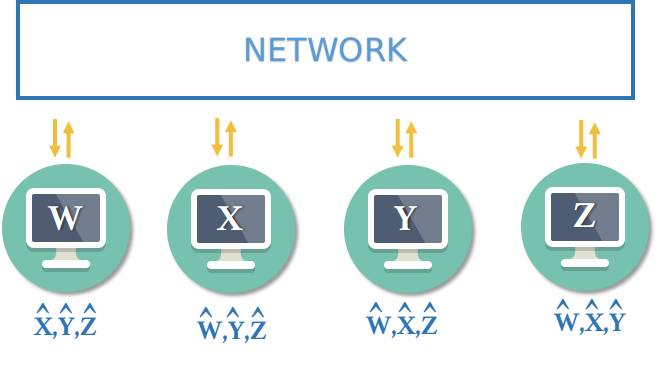
\includegraphics[scale=0.4]{./multipartydataex.png}
\label{fig:exitfun}
\end{center}
\end{figure}
Multiple parties observing correlated data seek to recover each other's data. How can they accomplish this using minimum communication?
\end{frame}

%-------------------Two party case
\begin{frame}[label = twoparty]
\frametitle{The Data-Exchange Problem}
\framesubtitle{Two party case}
\begin{minipage}[0.9\textheight]{\textwidth}
\begin{columns}
\begin{column}{0.4\textwidth}
\begin{itemize}
\item Random correlated data (X,Y) is distributed between two parties.
\item The first observes X and second observes Y.
\item They seek to recover each others data.
\item The joint distribution of X and Y is unknown.
\end{itemize}
\end{column}
\begin{column}{0.5\textwidth}
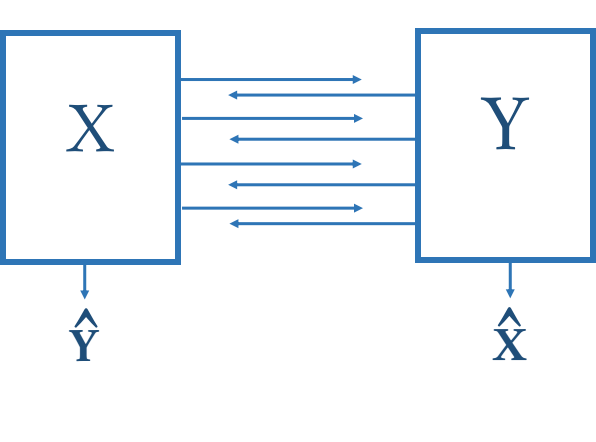
\includegraphics[width=5.2cm]{./dataexp.png}
\end{column}
\end{columns}
\end{minipage}\\
\vspace{0.5cm}
This project seeks to device a protocol which achieves this with minimal communication. 
\blfootnote{\tiny The order of communication is important in multiparty.}
\end{frame}

%----------------------rsynccomp
\begin{frame}[label= rsynccomp]
\frametitle{Working Solution}
\framesubtitle{r-sync vs Slepian-Wolf compression}
\begin{itemize}
\item In practice, algorithms like r-sync are used for data exchange.
\begin{itemize}
\item Uses \emph{one} guess.
\item Does not exploit the correlation between the data well.
\item Needs more communication.
\item Fast and low complexity.
\end{itemize}
\end{itemize}
\begin{minipage}[0.5\textheight]{\textwidth}
\begin{columns}
\begin{column}{0.4\textwidth}
\begin{itemize}
\item In theory, Slepian-Wolf compression is optimal. 
\begin{itemize}
\item $H(X|Y)$ is sufficient to estimate X from Y.
\end{itemize}
\end{itemize}
\end{column}
\begin{column}{0.5\textwidth}
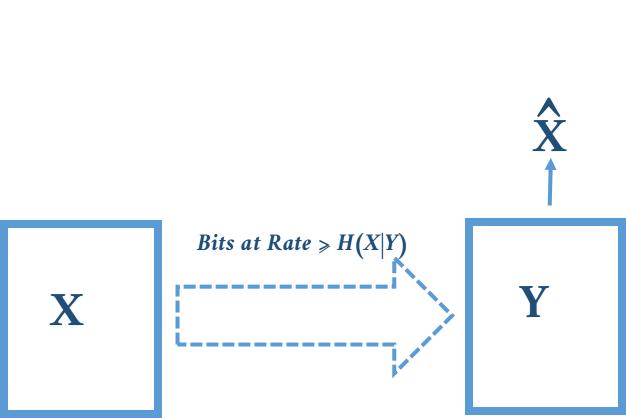
\includegraphics[width=5.2cm]{./swcompp.png}
\end{column}
\end{columns}
\end{minipage}
\hypercorner{\hyperlink{rsync}{\beamerbutton{r-sync}}}
\end{frame}

%--------------------implementation of slepian wolf
\begin{frame}
\frametitle{Implementation of SW compression.}
\framesubtitle{ Difficulties and suggested approach...}
Difficulties in implementation of SW compression
\begin{itemize}
\item Search is over an exponential list in decoding.
\item Knowledge of $P_{X|Y}$ is required at encoder.
\end{itemize}
\begin{block}{Suggested Approach}
\begin{itemize}
\item{Implement SW Compression using Polar Codes.}
\item{Achieve universality using \emph{recursive data exchange} protocol (RDE).}
\item{Realize RDE using Rateless Polar Codes with physical layer error detection.}
\end{itemize}
\end{block}
\end{frame}

%===========================Outline
\section{Outline}
\begin{frame}
\frametitle{Outline}
\begin{itemize}
\item Background
\begin{itemize}
\item{Recursive Data Exchange (RDE)}
\item{Brief introduction to Polar Codes}
\item{Slepian-Wolf compression with Polar Codes}
\item{Rateless Polar Codes}
\item{Rateless Polar Codes as HARQ}
\end{itemize}
\item Proposed implementation of RDE
\begin{itemize}
\item Adaptation of Rateless Polar Code for RDE
\item PHY-Layer error detection
\end{itemize}
\item Performance evaluation
\item Conclusion and future work
\end{itemize}
\end{frame}

%============================background
\section{Background}

%----------------------------RDE
\begin{frame}[label = rde]
\frametitle{Recursive Data Exchange (RDE)}
The \emph{recursive data exchange}\footnote{\tiny H. Tyagi and S. Watanabe, Universal Multiparty Data Exchange and Secret Key arrangement, \textit{ISIT,} 2016} protocol is based on an interactive version of the SW protocol
\begin{minipage}[0.9\textheight]{\textwidth}
\begin{columns}
\begin{column}{0.4\textwidth}
\begin{itemize}
\item This protocol is \emph{universal} as it does not rely on knowledge of the joint distribution.
\item The suggested decoders are theoretical constructs which are not implementable.
\end{itemize}
\end{column}
\begin{column}{0.5\textwidth}
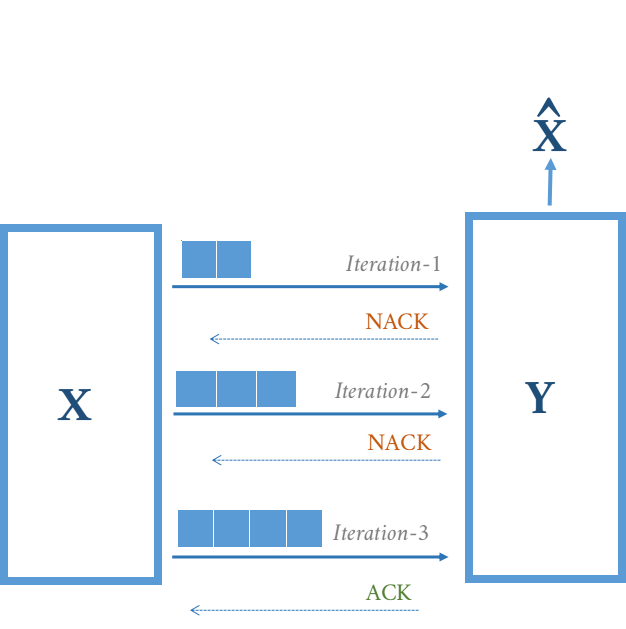
\includegraphics[width=5.2cm]{./rde.png}
\end{column}
\end{columns}
\end{minipage}\\
\end{frame}

%----------------------------Polar codes
\begin{frame}[label = polarcodes]
\frametitle{Brief Introduction to Polar Codes}
\framesubtitle{Channel polarization}
\begin{minipage}[0.9\textheight]{\textwidth}
\begin{columns}
\begin{column}{0.5\textwidth}
\begin{figure}
\centering
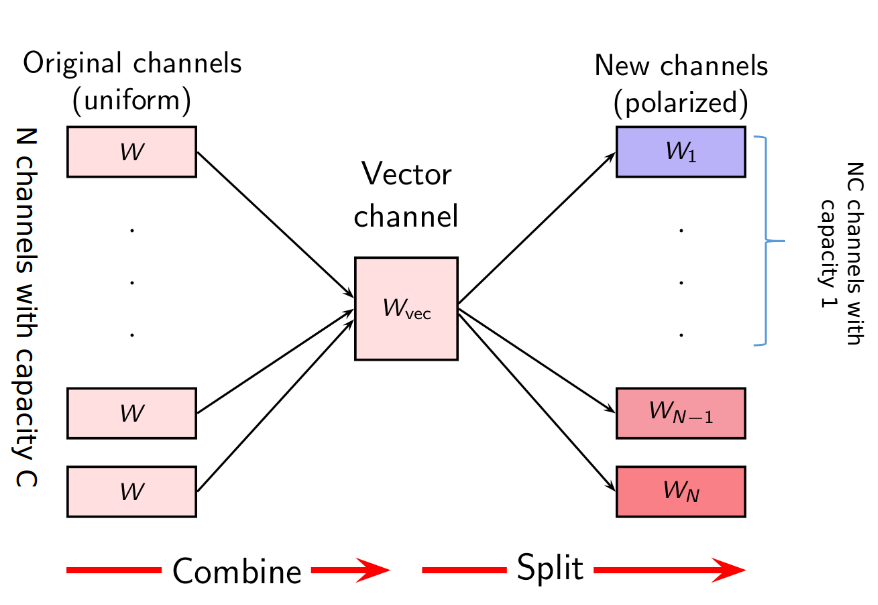
\includegraphics[width=5cm]{./channelcombp.png}
\end{figure}
\end{column}
\begin{column}{0.5\textwidth}
\begin{figure}
\centering
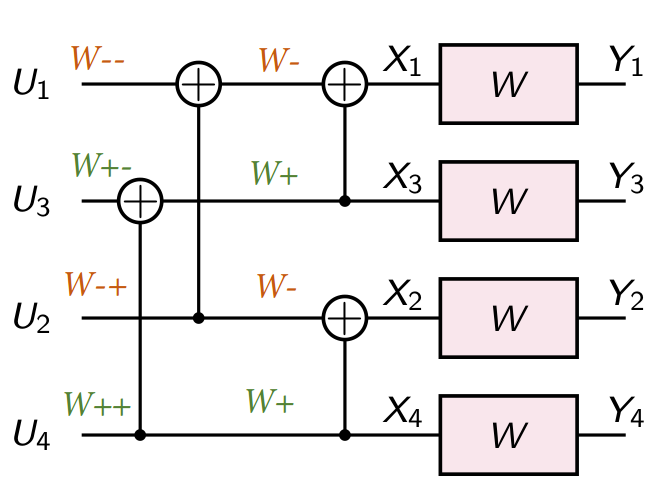
\includegraphics[width=4cm]{./arikanflyp4.png}
\end{figure}
\end{column}
\end{columns}
\end{minipage}
\begin{itemize}
\item $N$ independent copies of a given B-DMC ($W$) are combined and split into a second set of $N$ channels $\{W^{(i)}_N : 1 \leq i \leq N \}$.
\item There symmetric capacity $I(W^{(i)}_N )$ tend towards $0$ or $1$.
\item The channels with Bhattacharya parameter $Z(W^{(i)}_N)=0$ captures the capacity of $W_{vec}$.
\end{itemize}
\end{frame}

%----------------------polar encodedecode
\begin{frame}[label = polarencodedecode]
\frametitle{Brief Introduction to Polar Codes}
\framesubtitle{Encoding and decoding}
\begin{figure}
\centering
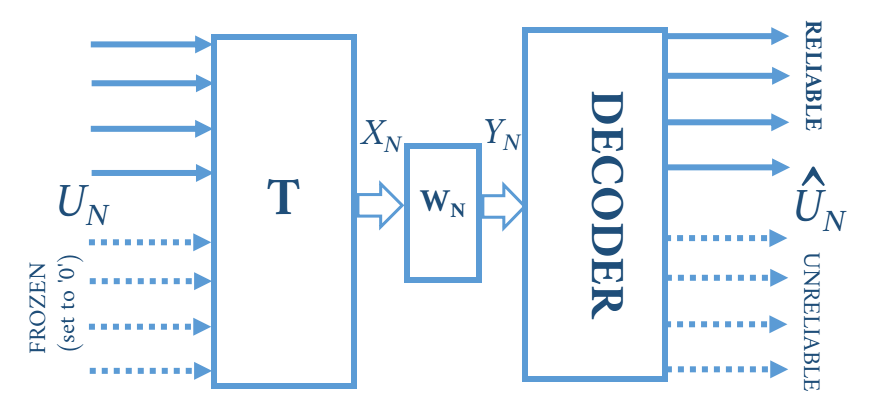
\includegraphics[width=7cm]{./pchschemep.png}
\end{figure}
\begin{itemize}
\item The encoding process\footnote{\tiny {$U_N$ is a uniform message vector, $T$ is a linear transform for the butterfly.}} sends data on transformed channels with $Z(W^{(i)}_N)=0$  (\emph{good channels}) and treats the channels with $Z(W^{(i)}_N)=1$ as \emph{frozen}, sending no useful data on them.
\item For our purpose, we shall be using Successive Cancellation (SC) decoding.
\end{itemize}
\hypercorner{\hyperlink{polarencode}{\beamerbutton{Encoding}} \hyperlink{polardecode}{\beamerbutton{SC-Decoding}} \hyperlink{polarperformance}{\beamerbutton{Performance}}}
\end{frame}

%----------------------polar slepian
\begin{frame}[label = polarslepian]
\frametitle{Slepian-Wolf compression with Polar Codes}
\begin{figure}
\centering
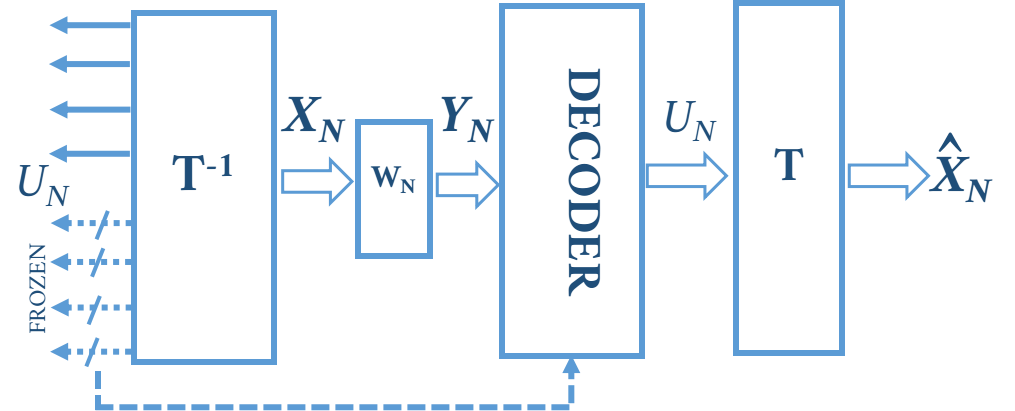
\includegraphics[width=7cm]{./pswschemep.png}
\end{figure}
\begin{itemize}
\item $Y_N$ is a corrupted version of $X_N$ by $N$ BSC(p) channels.
\item The bits that are to be sent for estimation of $X_N$ from $Y_N$ are the frozen bits in $U_N$. This is the data compression operation. 
\item These bits are communicated error free to the SC-decoder. 
\item $H(X_N)-I(W_N)=H(X_N/Y_N)$ bits are sent. 
\end{itemize}
\blfootnote{\tiny S. Onay.Polar Codes for Nonassymetric Slepian-Wolf
Coding.arXiv.1208.3056v1[cs.IT], August 2012.}
\hypercorner{ \hyperlink{polarswperformance}{\beamerbutton{Performance}}}
\end{frame}
%---------------------Rateless polar codes
\begin{frame}[label = rpc]
\frametitle{Rateless Polar Codes}
\framesubtitle{Rateless code}
\begin{block}{Rateless Code}
A rateless coding scheme transmits incrementally more and more coded bits over an unknown channel until all the information bits are decoded reliably by the receiver.
\end{block}
\begin{itemize}
\item A rateless code is designed for a set of channels and judged for its performance for the entire set.
\item In general rateless code design is based on Hybrid-ARQ techniques and uses code puncturing.
\item Rateless Polar Codes can be constructed using nesting property of Polar Codes for degraded channels.
\end{itemize}
\end{frame}
%---------------------degradedness and nesting
\begin{frame}[label = dgnest]
\frametitle{Rateless Polar Codes}
\framesubtitle{Degraded channels and nesting property}
\begin{columns}
\begin{column}{0.6\textwidth}
\begin{block}{Degraded channels} 
if X\---Y\---Z, and $W_1=P_{Y|X}$, $W_2=P_{Z|X}$ then $W_2 \preceq W_1$.
\end{block}
\begin{itemize}
\item The capacity of $W_2$ is lesser than that of $W_1$. $W_2$ has lesser number of good channels.
\item e.g., $BSC(p_1) \preceq BSC(p_2)$ if $p_1 \geq p_2$.
\end{itemize}
\end{column}
\begin{column}{0.3\textwidth}
\begin{figure}
\centering
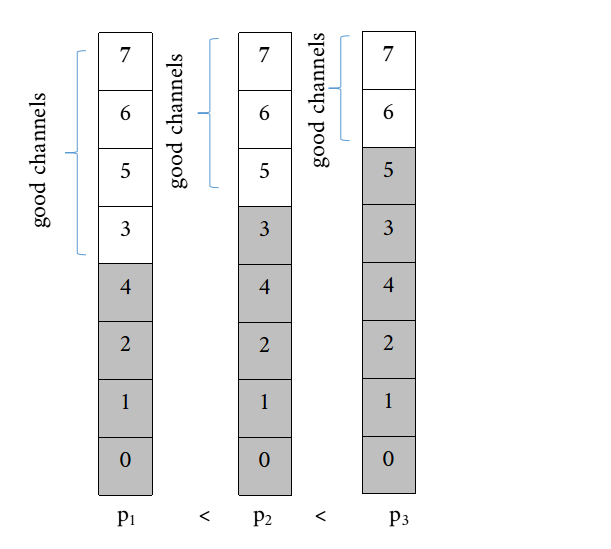
\includegraphics[width=5cm]{./relorder.png}
\end{figure}
\end{column}
\end{columns}
\begin{itemize}
\item The good bit indices of $W_2$ is a subset of the good bit indices of $W_1$.\footnote{\tiny E. Sasoglu and L. Wang. Universal Polarization. arXiv:1307.7495v2[cs.IT], Dec.
2013.}
\item  A more reliable bit-channel is always noiseless if a less reliable bit-channel is noiseless. This leads to \emph{reliability ordering}.
\end{itemize}
\end{frame}
%--------------------------------------IncFrz
\begin{frame}[label = incfrz]
\frametitle{Incremental Freezing}
\framesubtitle{Rateless Polar Code employing reliability ordering}
\begin{figure}
\centering
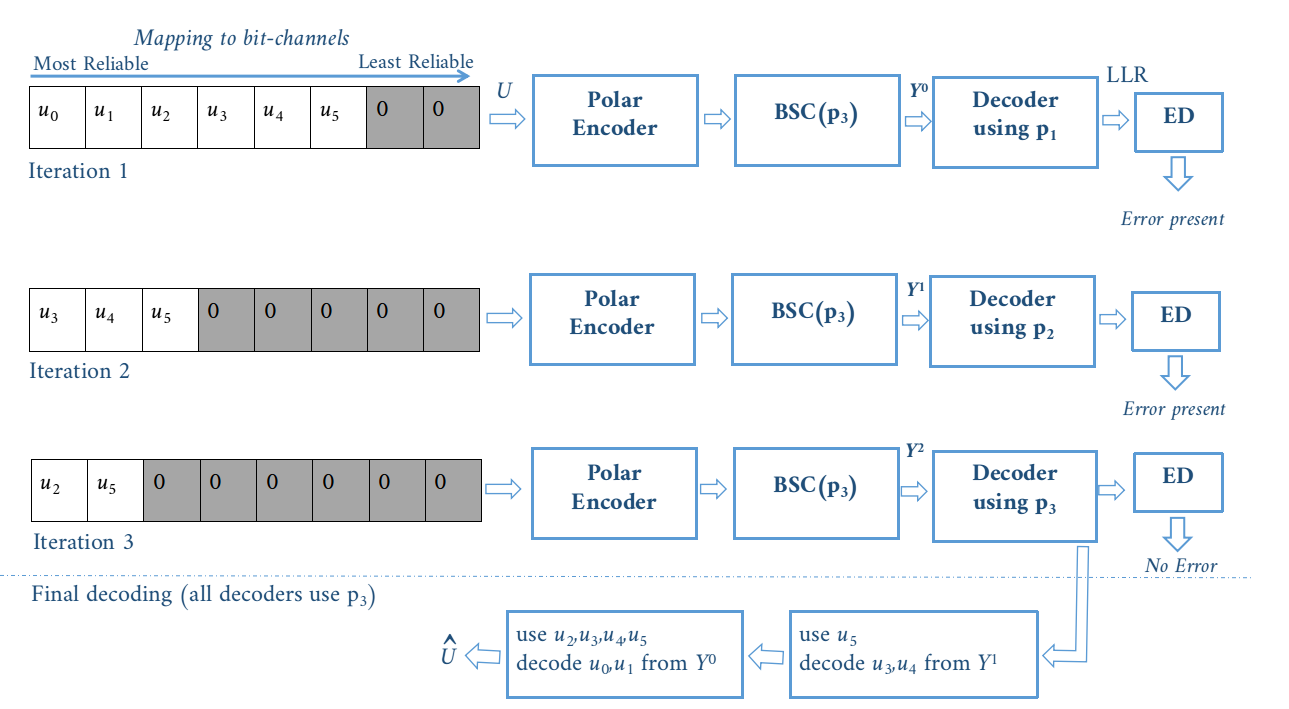
\includegraphics[width=9cm]{./ifp.png}
\end{figure}
\begin{itemize}
\item Initial transmission is done using a high rate Polar Code.
\item If decoding fails then the comparatively lesser reliable channels are retransmitted.  
\end{itemize}
\hypercorner{\hyperlink{incfrz2}{\beamerbutton{more info...}}}
\blfootnote{\tiny M. Mondelli et al. Capacity achieving rate compatible polar codes for general channels, Jan. 2017.}
\end{frame}

%------------------------------HARQ
\begin{frame}[label = HARQ]
\frametitle{Rateless Polar Codes as Hybrid ARQ}
\begin{itemize}
\item In standard ARQ, redundant bits are added to data to be transmitted using an error-detecting (ED) code such as a cyclic redundancy check (CRC). \item Receivers detecting a corrupted message will request a new message from the sender. 
\end{itemize}
\begin{block}{Hybrid -ARQ}
In Hybrid ARQ, the original data is encoded with a forward error correction (FEC) code, and the parity bits are only transmitted upon request when a receiver detects an erroneous message (Type-II). 
\end{block}
\begin{itemize}
\item Construction of HARQ requires the following,
\begin{itemize}
\item Rate Compatible Code 
\item A choice of retransmission vector (RV).
\end{itemize}
\end{itemize}
\hypercorner{ \hyperlink{rcp}{\beamerbutton{Rate Compatible Codes}}}
\end{frame}
%------------------------------HARQ
\begin{frame}[label = HARQp]
\frametitle{Rateless Polar Codes as Hybrid ARQ}
\framesubtitle{H-ARQ for Polar Codes}
\begin{itemize}
\item Polar Codes for degraded channels are inherently rate compatible due to reliability ordering and nesting.
\item The choice of RV may be based on,
\\
\begin{itemize}
\item Selective Repetition of unreliable bits.
\item Incremental Freezing.
\item Subset Polar codes.
\end{itemize}
\vspace{.5cm}
\item The ED code may be omitted using Reliability based H-ARQ.
\begin{itemize}
\item Reliability based HARQ uses the soft outputs (LLR) of the decoder to perform ED.
\end{itemize}
\end{itemize}
\hypercorner{ \hyperlink{selrep}{\beamerbutton{Selective Repetition}} \hyperlink{subpol}{\beamerbutton{Subset Polar Codes}} \hyperlink{rbharq}{\beamerbutton{RB-HARQ}}}
\end{frame}

%=========================Proposed solution
\section{Proposed solution}
%------------------------------proposed solution
\begin{frame}[label=propsol]
\frametitle{Proposed Solution}
\textit{Our approach towards implementation of a solution to the \emph{Data-Exchange} problem using RDE and Polar Codes ... }
\begin{block}{Proposed implementation of RDE}
\begin{itemize}
\item{Use Rateless Polar Codes with Incremental Freezing to implement RDE.}
\item{Use a PHY layer error detection as retransmission criterion in Incremental Freezing.}
\end{itemize}
\end{block}
\end{frame}
%----------------------Adaptation
\begin{frame}[label=adapt0]
\frametitle{Adaptation of Rateless Polar Codes for RDE}
\framesubtitle{Setting}
\begin{figure}[h]
 \begin{center}
    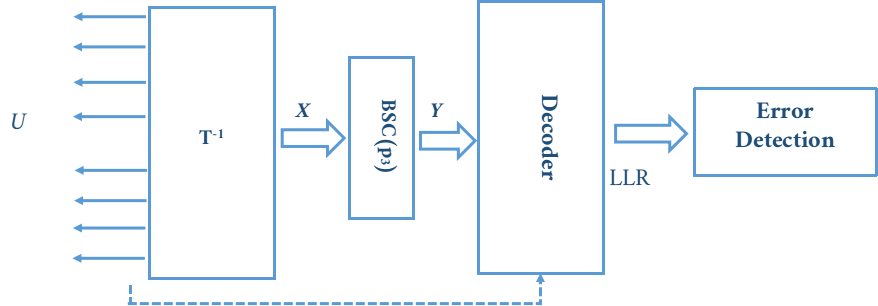
\includegraphics[width=7cm]{setting.png}
  \end{center}
  \label{fig:iswrpc}
\end{figure} 
\begin{itemize}
\item Consider, a compound BSC channel $\mathcal{C}=\{ p_1 \leq p_2 \leq p_3 \leq p_4\}$. where $p_i$ is the flipover probability of channel $i$. 
\item The rates supported by the channels are $\{ R_1=R, R_2= R/2,R_3= R/3,R_4= R/4\}$.
\item The actual channel is BSC($p_3$). We shall denote this as BSC($p_{channel}$).
\item The vector channel is manufactured by polarization of $N$ such BSC($p_{channel}$) channels.
\end{itemize}
\end{frame}

\begin{frame}[label=adapt1]
\frametitle{Adaptation of Rateless Polar Codes for RDE}
\begin{figure}[h]
 \begin{center}
    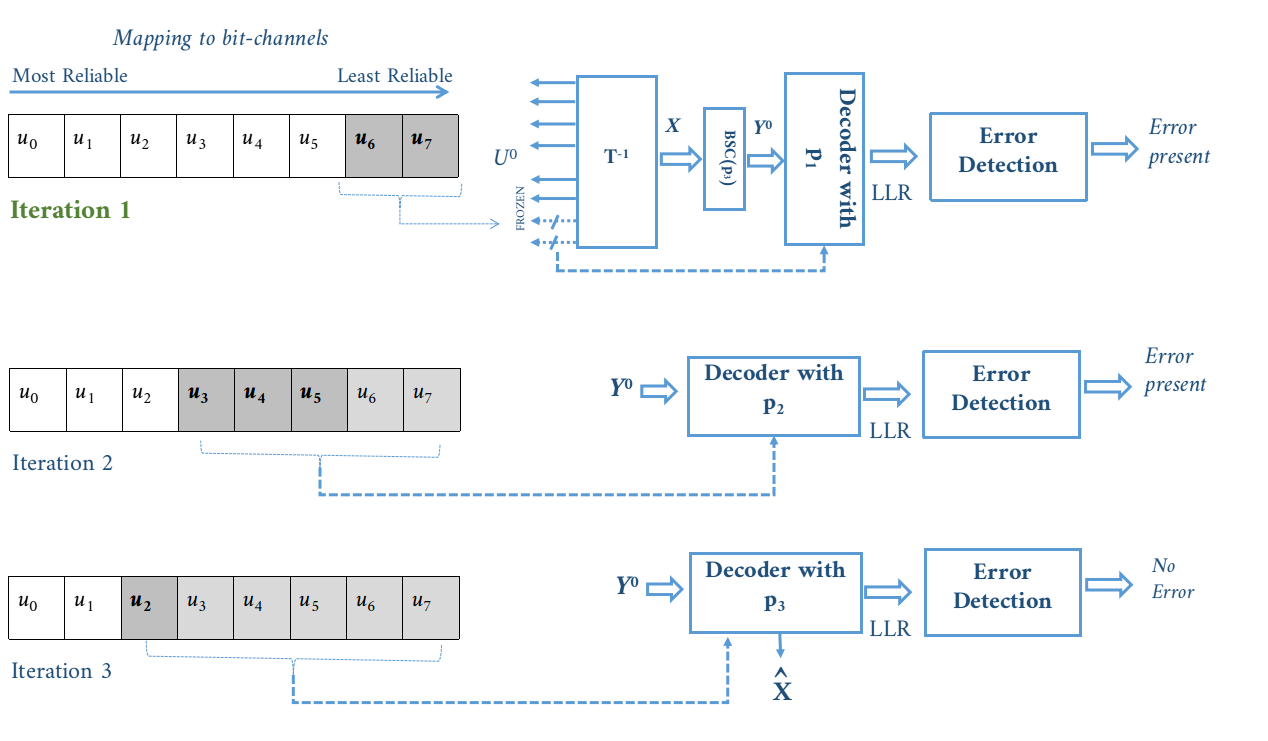
\includegraphics[width=9cm]{iswrpcp1.png}
  \end{center}
  \label{fig:iswrpc}
\end{figure} 
\begin{itemize}
\item In the first iteration the encoder and decoder \emph{guesses} the channel to be BSC($p_1$) greedily.
\item The encoder sends the corresponding frozen bits to decoder error-free.
\item The decoder computes $|LLR|$ using BSC($p_1$) and performs ED.
\item In case of error (as here) receiver replies with a NACK.
\end{itemize}
\end{frame}

\begin{frame}[label=adapt2]
\frametitle{Adaptation of Rateless Polar Codes for RDE}
\begin{figure}[h]
 \begin{center}
    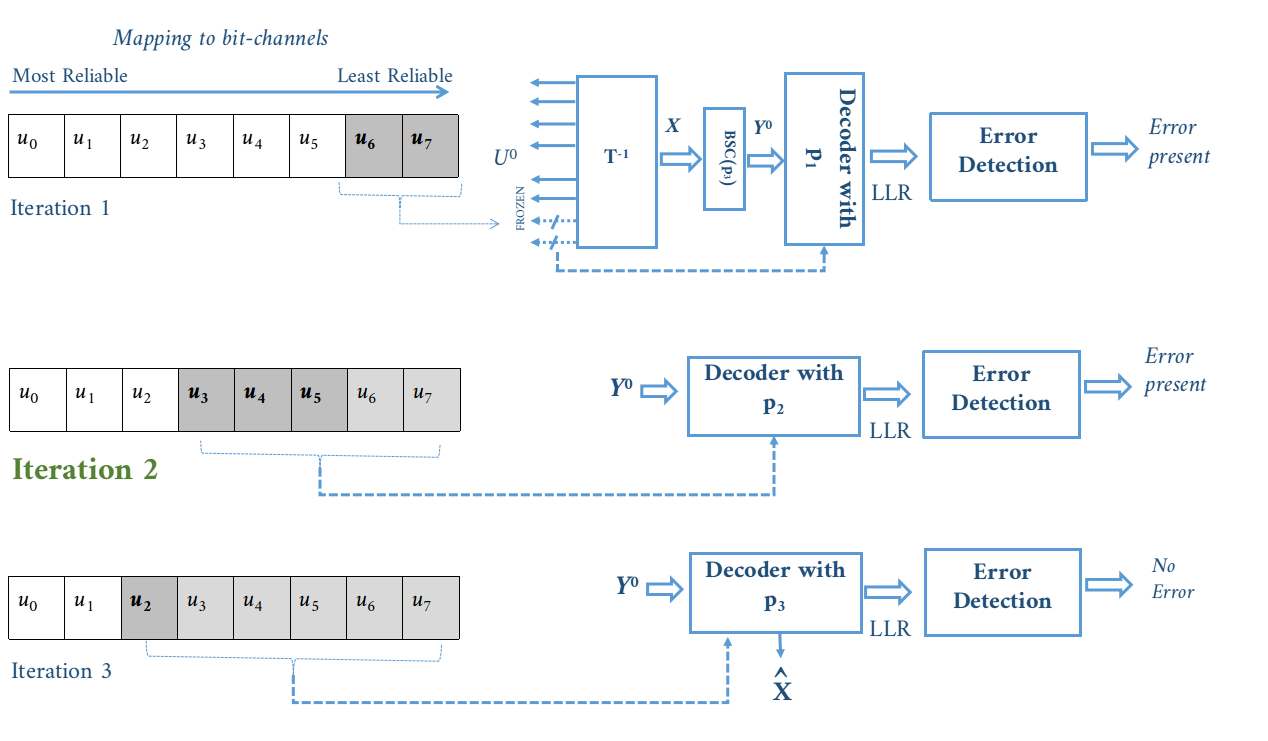
\includegraphics[width=9cm]{iswrpcp2.png}
  \end{center}
  \label{fig:iswrpc}
\end{figure}
\begin{itemize}
\item In the second iteration $p_{guess}=p_2$.
\item The error-free transmission in this iteration consist of information bits which are reliable if $p_{channel}=p_1$ but unreliable if $p_{channel}=p_2$.
\item The decoder replies with NACK.
\end{itemize}
\end{frame}

\begin{frame}[label=adapt3]
\frametitle{Adaptation of Rateless Polar Codes for RDE}
\begin{figure}[h]
 \begin{center}
    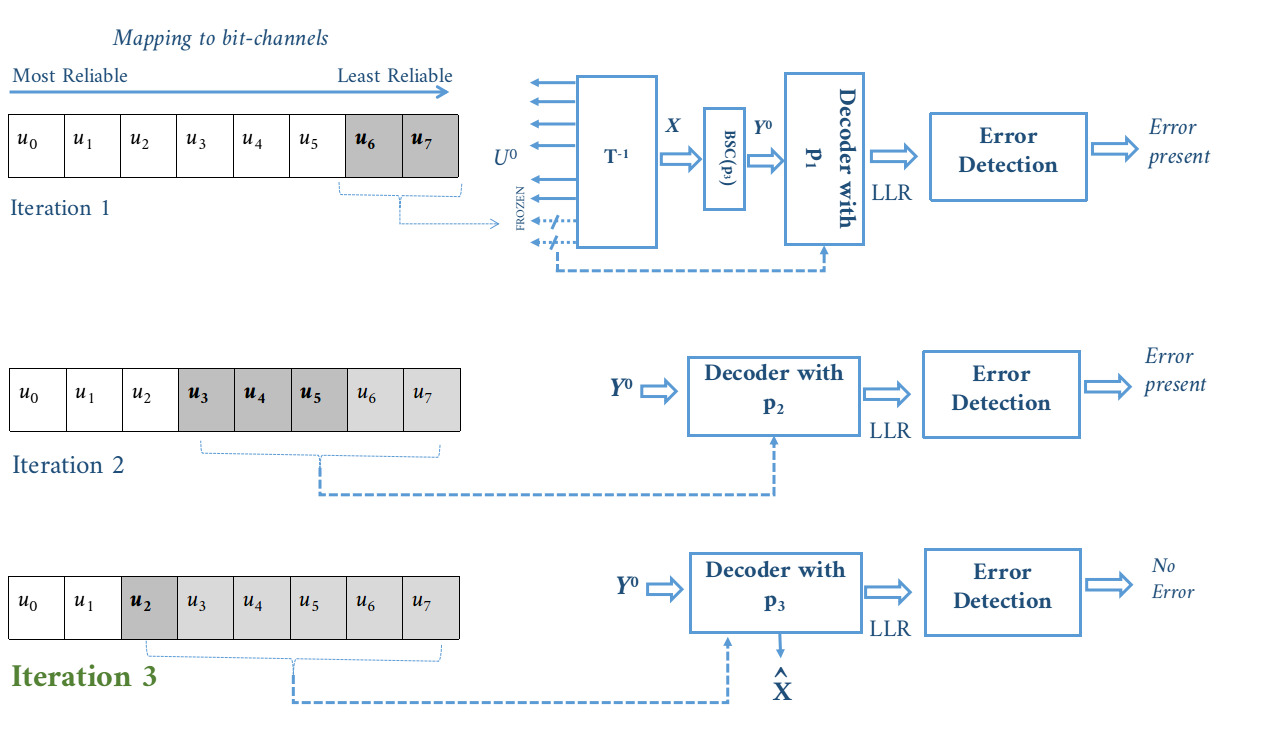
\includegraphics[width=9cm]{iswrpcp3.png}
  \end{center}
  \label{fig:iswrpc}
\end{figure}
\begin{itemize}
\item In the third iteration $p_{guess}=p_3=p_{channel}$.
\item The ED declares no error and replies with ACK. 
\item The decoder now  decodes the received channel output vector using $p_3$ and considering the bits transmitted error-free in \emph{all} the iterations as frozen. Finally, with Arikan transform X is estimated.
\end{itemize}
\end{frame}
%------------------------------------PHY-ED
\begin{frame}[label=phyed]
\frametitle{PHY-Layer Error Detection}
\begin{itemize}
\item In Polar Codes for error control CRC in $U_N$ can be exploited for ED.
\item In SW-compression with Polar Codes $U_N$ is generated from $X_N$.
\begin{itemize}
\item Hence, CRC cannot be used.
\item PHY-Layer ED is required as retransmission criterion.
\end{itemize}
\end{itemize}
\begin{block}{PHY-ED as hypothesis test}
Since Inc-Frz guesses the best channel first, we can say that at $j^{th}$ iteration $p_{guess}=p_j$. 
Error detection may be seen as a hypothesis test in \emph{each iteration} where,
\begin{align*}
\mathcal{H}_0 & :\text{The channel is the current guess, i.e., } j=i\\
\mathcal{H}_1 & :\text{The channel is worse, i.e., }j<i
\end{align*}
\vspace{0.1cm}
\end{block}
\vspace{0.5cm}
\tiny Note, $\mathcal{C}=\{ p_1 \leq p_2 \leq p_3 \leq p_4\}$.
\end{frame}
%---------------------------observables
\begin{frame}[label=obs]
\frametitle{PHY-Layer Error Detection}
\begin{block}{Observable}
Let $\Lambda_j^i(k)$ be the magnitude of the LLR of $k^{th}$ bit-channel, $k\in{1,2,...N}$ at the output of the decoder at the end of $j^{th}$ iteration such that $p_{guess}=p_j$ for $p_{channel}=p_i$.\\ $\Lambda_j^i(k)$ serve as the observables of the test after $j^{th}$ iteration.
\end{block}
\begin{figure}[h]
 \begin{center}
    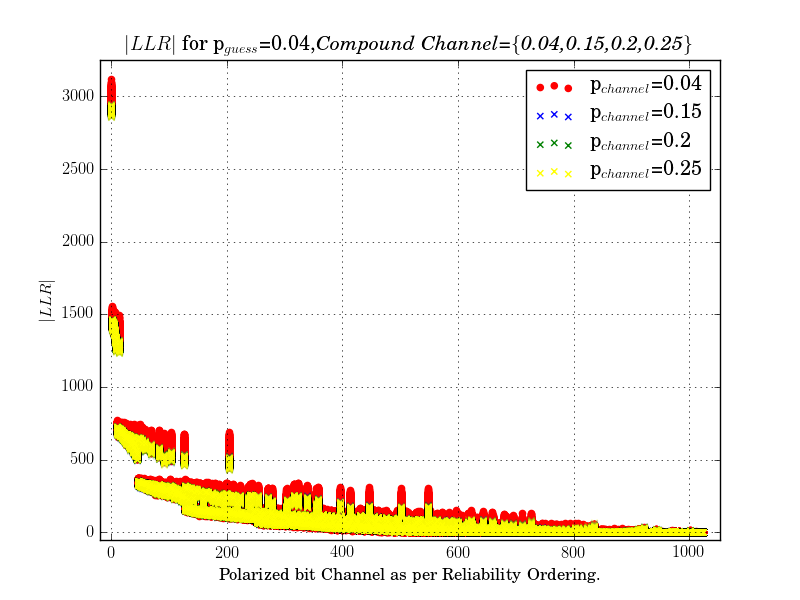
\includegraphics[width=6.5cm]{absllr0p04.png}
  \end{center}
  \label{fig:iswrpc}
\end{figure}
\end{frame}
%---------------------------tests
\begin{frame}[label=test1]
\frametitle{PHY-Layer Error Detection}
\framesubtitle{Proposed tests}
Let there be $K$ good bit-channels after polarization.  
\begin{block}{Test 1: All good channels are above a given threshold.}
Initially, a test was considered where $p_{guess}=p_{channel}$ is declared if the $|LLR|$ of all the good channels clear a given threshold under the current guess. That is, after $j^{th}$ iteration,
\begin{align*}  
j & =i, 
\begin{cases}
\text{   if, }  \Lambda_{j}^i(k) > \lambda, \forall k \in {1,2,3...K}\\
\text{alternatively, } \displaystyle\min_{k \in [K]}\Lambda_{j}^i(k) > \lambda  \\
\end{cases}\\
 j & < i,  \text{ o.w.}
\end{align*} 
\end{block}
\small
The support of the distributions of $\Lambda_{j=i}^i(k)$ and $\Lambda_{j \neq i}^i(k)$ overlap considerably and $\Lambda_{j=i}^i(k)$ has a higher variance.
This gave rise to high missed detection probability $P_M$\footnote{\tiny $P_M$ indicates the probability that the test declares a better channel as the true channel.}
\end{frame}

\begin{frame}[label=test2]
\frametitle{PHY-Layer Error Detection}
\framesubtitle{Proposed tests}
\begin{block}{Test 2: A given fraction of good channels are above a threshold.}
In this test $p_{guess}=p_{channel}$ is declared if the $|LLR|$ of a certain fraction of the good channels clear a threshold. The fraction is dependent on the iteration number. After $j^{th}$ iteration,
\begin{align*}  
j &=i,
 \text{   if, } \frac{1}{K}\sum^K_{k=1} \mathbbm{1}_{\{\Lambda_{j}^i(k) > \lambda\}} > \Theta_j \\
j & < i,  \text{ o.w. }
\end{align*} 
\end{block}
\end{frame}
%-------------------------------------theta
\begin{frame}[label=theta1]
\frametitle{PHY-Layer Error Detection}
\framesubtitle{$P_M$ and $P_F$ for Test 2}
\begin{figure}[h]
 \begin{center}
    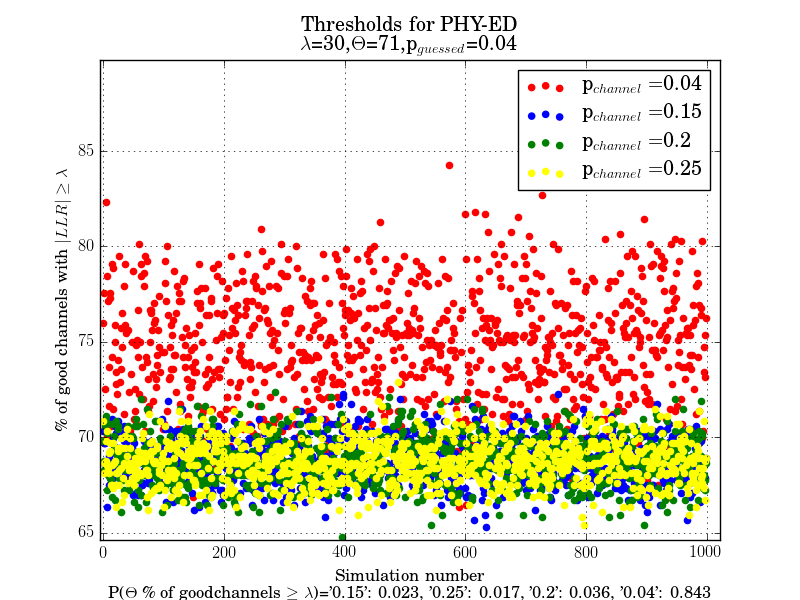
\includegraphics[width=8cm]{theta0p04.png}
  \end{center}
  \label{fig:iswrpc}
\end{figure}
From figure, the detection error probabilities for the first  iteration can be calculated as $P_F=0.16$ and $P_M=0.06$.
\end{frame}

\begin{frame}[label=theta2]
\frametitle{PHY-Layer Error Detection}
\begin{itemize}
\item A higher value of $P_M$ affects frame error probabilities adversely.
\item A higher value of $P_F$ does not affect the frame error probabilities but causes rate loss. 
\end{itemize}
\begin{minipage}[1.1\textheight]{\textwidth}
\begin{columns}
\begin{column}{0.5\textwidth}
\begin{figure}
\centering
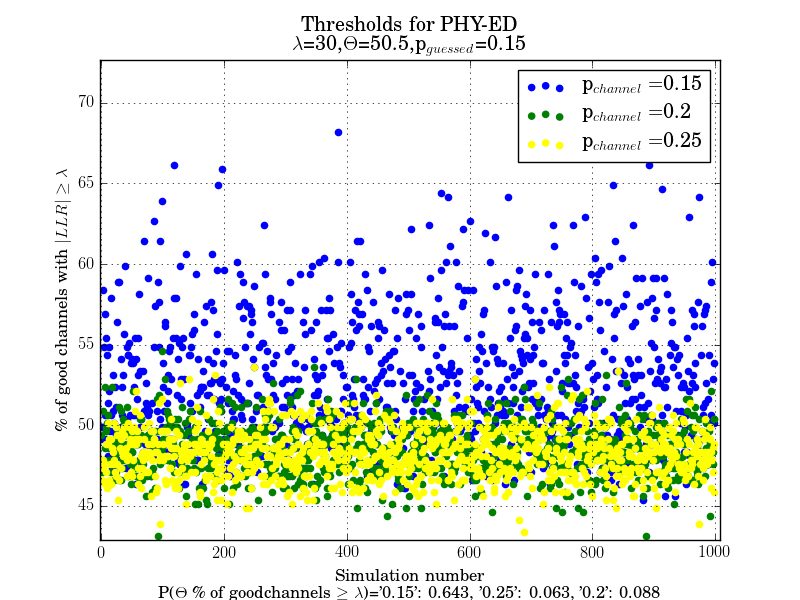
\includegraphics[width=6cm]{./theta0p15new.png}
\end{figure}
\end{column}
\begin{column}{0.5\textwidth}
\begin{figure}
\centering
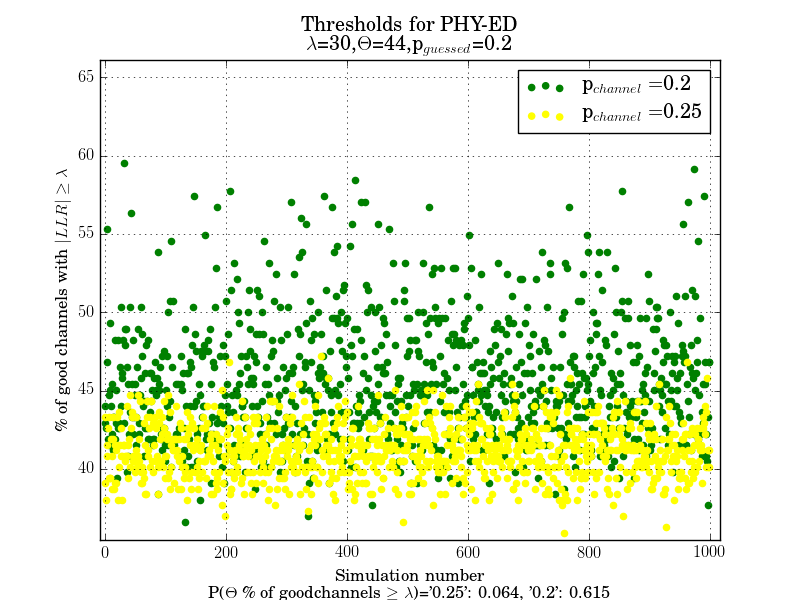
\includegraphics[width=6cm]{./theta0p2.png}
\end{figure}
\end{column}
\end{columns}
\vspace{0.5cm}
\small $P_F\approx0.4$  for second and third iteration with $P_M\approx0.13$.
\end{minipage}
\end{frame}
%======================================Performance evaluation
\section{Performance evaluation}
\begin{frame}[label=psw1]
\frametitle{Performance Evaluation}
Let $K$ be the number of bit-channels assumed to be good at the first iteration. For simulation, $K$ is varied from $0$ to $K^*$ such that $K^*/N$ is the capacity of the best channel. In case of SW compression the number of bits that remain unfrozen after the final iteration divided by $N$ is viewed as the achieved rate.
\begin{minipage}[1.1\textheight]{\textwidth}
\begin{columns}
\begin{column}{0.5\textwidth}
\begin{figure}
\centering
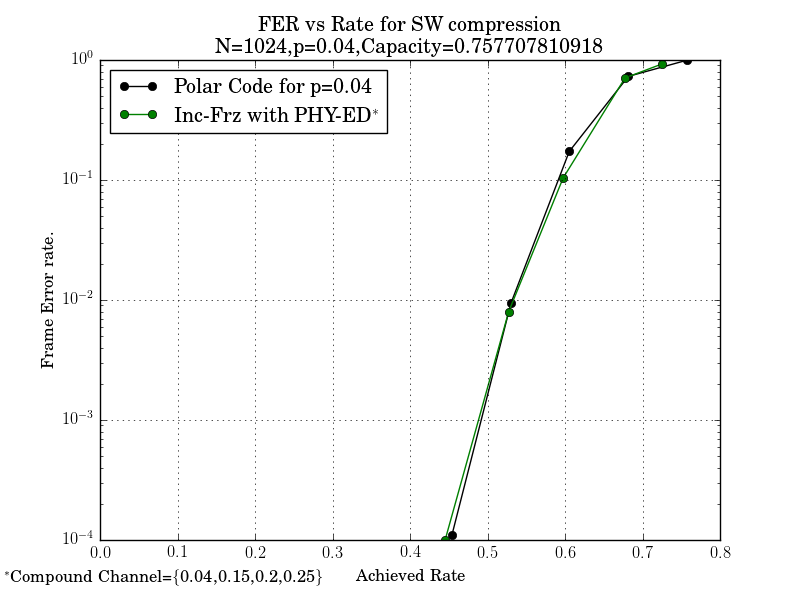
\includegraphics[width=6cm]{./FERSW_0p04.png}
\end{figure}
\end{column}
\begin{column}{0.5\textwidth}
\begin{figure}
\centering
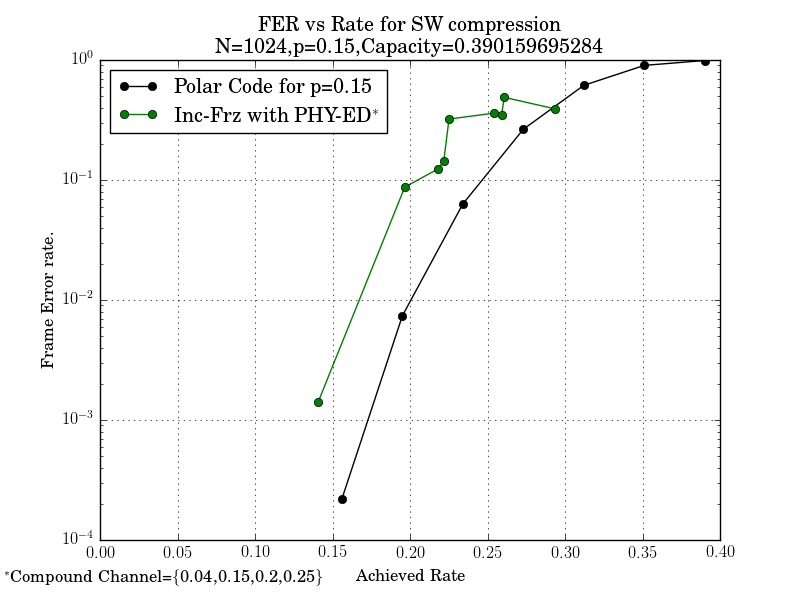
\includegraphics[width=6cm]{./FERSW_0p15.png}
\end{figure}
\end{column}
\end{columns}
\end{minipage}
\hypercorner{\hyperlink{pch1}{\beamerbutton{EC-performance}}}
\end{frame}

\begin{frame}[label=psw2]
\frametitle{Performance Evaluation}
\begin{minipage}[1.1\textheight]{\textwidth}
\begin{columns}
\begin{column}{0.5\textwidth}
\begin{figure}
\centering
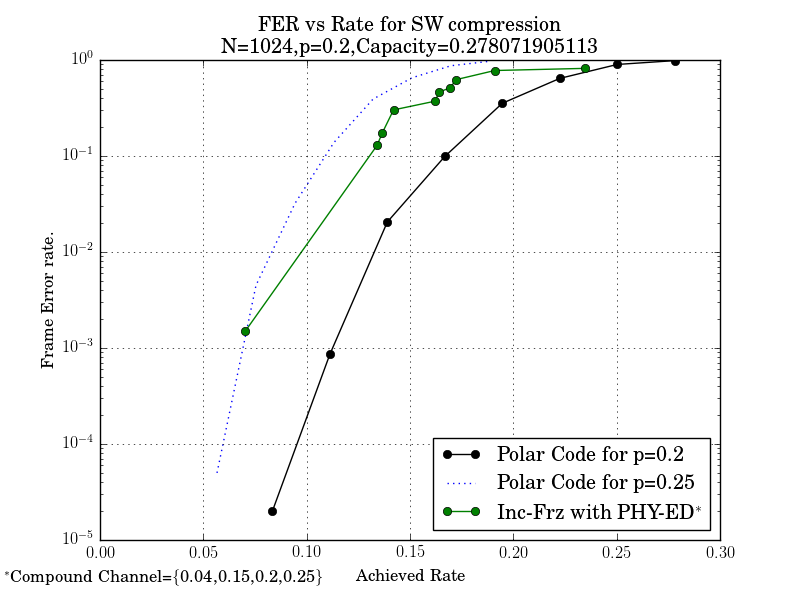
\includegraphics[width=6cm]{./FERSW_0p2.png}
\end{figure}
\end{column}
\begin{column}{0.5\textwidth}
\begin{figure}
\centering
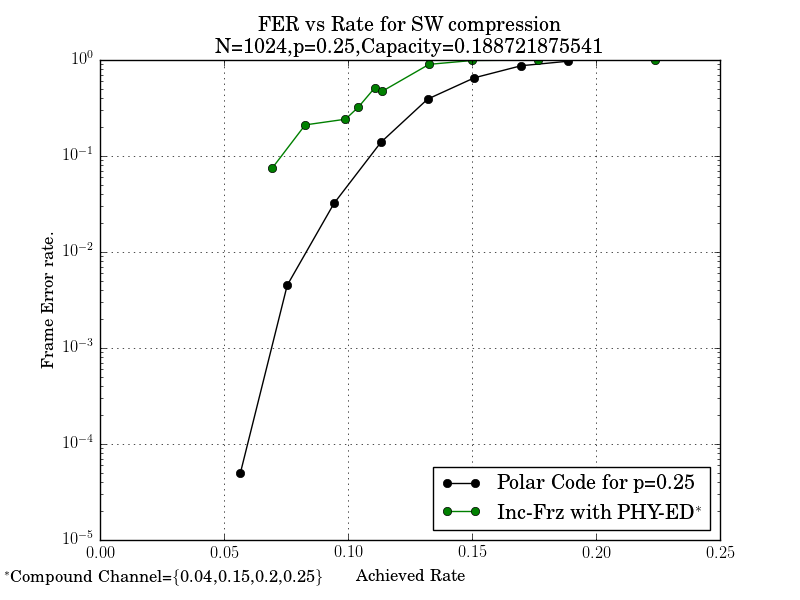
\includegraphics[width=6cm]{./FERSW_0p25.png}
\end{figure}
\end{column}
\end{columns}
\end{minipage}
\hypercorner{\hyperlink{pch2}{\beamerbutton{EC-performance}}}
\end{frame}

\begin{frame}[label=psw3]
\frametitle{Performance Evaluation}
\begin{figure}
\centering
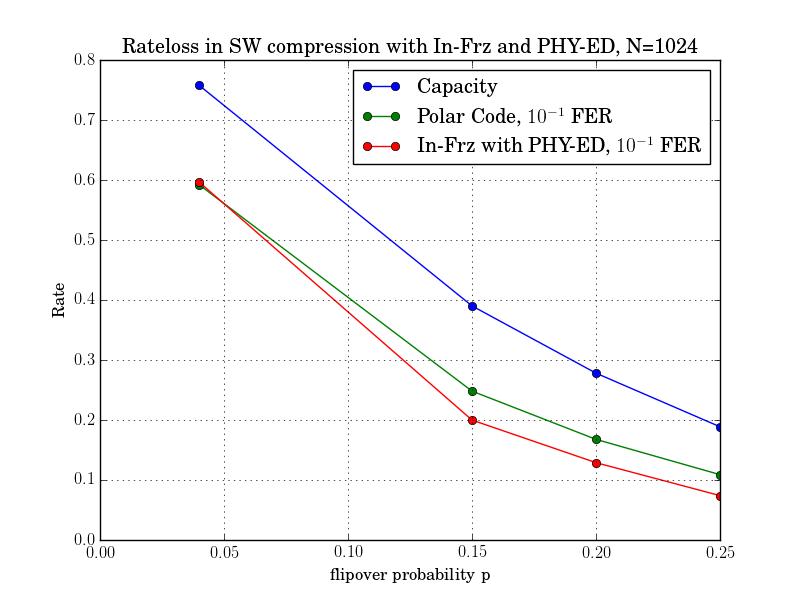
\includegraphics[width=9cm]{./ratelosssw.png}
\end{figure}
\hypercorner{\hyperlink{pch3}{\beamerbutton{EC-performance}}}
\end{frame}

%=====================================Conclusion
\section{conclusion}
\begin{frame}[label=conc]
\frametitle{Conclusion and Future work}
\begin{itemize}
\item The proposed scheme is an implementable solution to the \emph{Data-Exchange} problem.
\item It reduces the communication among nodes.
\item The CRC-free universal polar code promises considerable rate gain for communication using short packet lengths. 
\item There are few channels which are good for use during the entire transmission. Communicating critical data over these channel ensure high reliability and availability . 
\end{itemize}
\begin{itemize}
\item Future work.
\begin{itemize}
\item Extensive performance analysis and theoretical analysis of proposed error detection scheme as a RB-HARQ for Polar Codes.
\item Implementation of the scheme for multiparty data exchange.
\end{itemize}
\end{itemize}
\end{frame}

%%===================================reference
%\section{Bibliography}
%\begin{frame}{References}
%\begin{enumerate}
%\item[(1)] S. Kumar and H. D. Pfister, “Reed-Muller codes achieve
%capacity on erasure channels,” 2015, [Online]. Available:
%http://arxiv.org/abs/1505.05123v2.
%\item[(2)] S. Kudekar, M. Mondelli, E. \c{S}a\c{s}\u{o}glu, and R. Urbanke, “Reed-Muller codes achieve capacity on the binary erasure channel under MAP
%decoding,” 2015, [Online]. Available: http://arxiv.org/abs/1505.05831v1.
%\item[(3)] {\color{MidnightBlue}$\equiv (1) \cup (2)$} S. Kudekar, S. Kumar, M. Mondelli, H. D. Pfister, E. \c{S}a\c{s}\u{o}glu, and R. Urbanke, “Reed-Muller codes achieve
%capacity on erasure channels,” 2016, [Online]. Available:
%http://arxiv.org/abs/1601.04689v1.
%\end{enumerate}
%\end{frame}

%=========================Thanks
\section{Questions}
\begin{frame}
\centering
\Huge Thank You!
\end{frame}

%============================Backup slides
\appendix
\section{Appendix}
%---rsync
\begin{frame}[label = rsync]
\frametitle{The r-sync protocol }
\begin{figure}
\centering
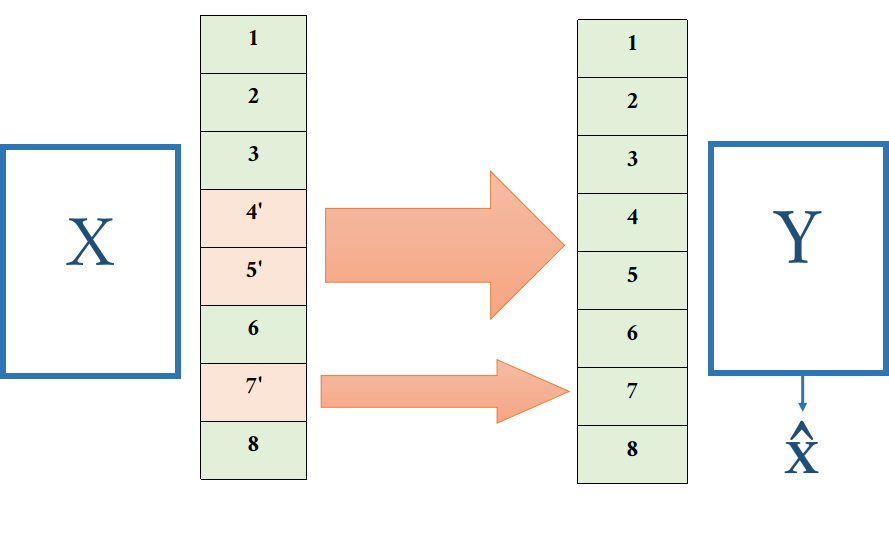
\includegraphics[width=9cm]{./rsync.png}
\end{figure}
\begin{itemize}
\item Files are divided into blocks and there hashes are compared.
\item The blocks with hash mismatch are transmitted.
\end{itemize}
\tiny For details see A. Tridgell and P. Mackerras. The r-sync algorithm. Joint Computer Science and
Technical Report Series, TR-CS-96-05, 1996.
\hypercorner{\hyperlink{rsynccomp}{\beamerbutton{back}}}
\end{frame}
%---polar encoding
\begin{frame}[label = polarencode]
\frametitle{Polar Encoding}
\begin{figure}
\centering
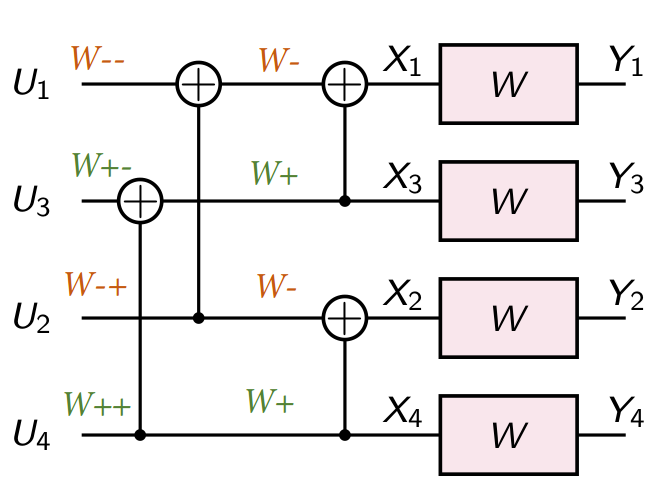
\includegraphics[width=6cm]{./arikanflyp4.png}
\end{figure}
$$X_N=U_N*F^{\otimes n}\text{,where } N=2^n$$ 
\[
F=
  \begin{bmatrix}
    1 & 0 \\
    1 & 1
  \end{bmatrix}
\]
$$\text{set }U_1=U_2=0$$
\hyperback{\hyperlink{polarencodedecode}{\beamerbutton{back}}}
\end{frame}
%-----polar decode
\begin{frame}[label = polardecode]
\frametitle{Succesive Cancellation Decoding}
\begin{figure}
\centering
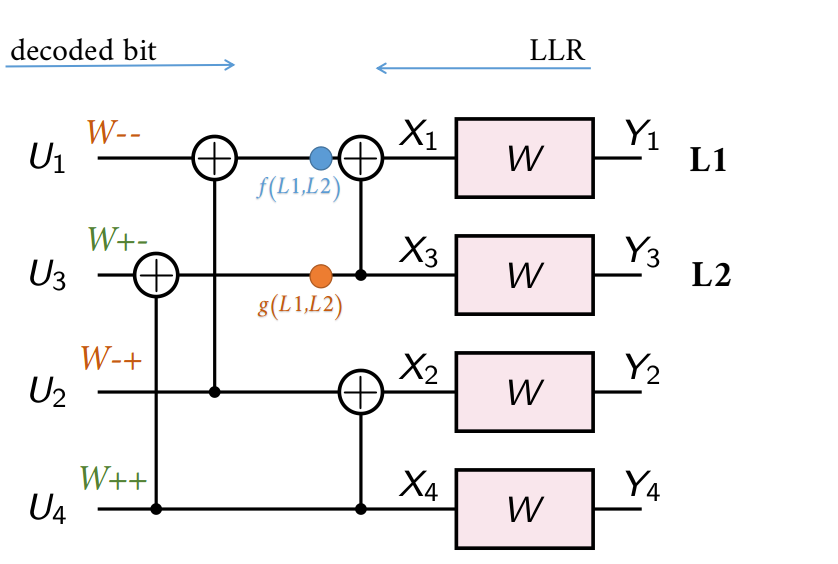
\includegraphics[width=6cm]{./scdecode.png}
\end{figure}
\begin{itemize}
\item Worse channels are decoded first. 
\item $f(L_1,L_2)=\frac{L_1*L_2+1}{L_1+L_2}$
\item $g(L_1,L_2)=L_1*L_2 \text{, if bit at }f\text{ is '}1\text{', else }L_2/L_1$
\item if bit is frozen, frozen value is used, else decoding is based on $f$ or $g$.
\end{itemize}
\hyperback{\hyperlink{polarencodedecode}{\beamerbutton{back}}}
\end{frame}
%-----------------------polar performance
\begin{frame}[label = polarperformance]
\frametitle{Performance of Polar Codes for error control}
\begin{figure}
\centering
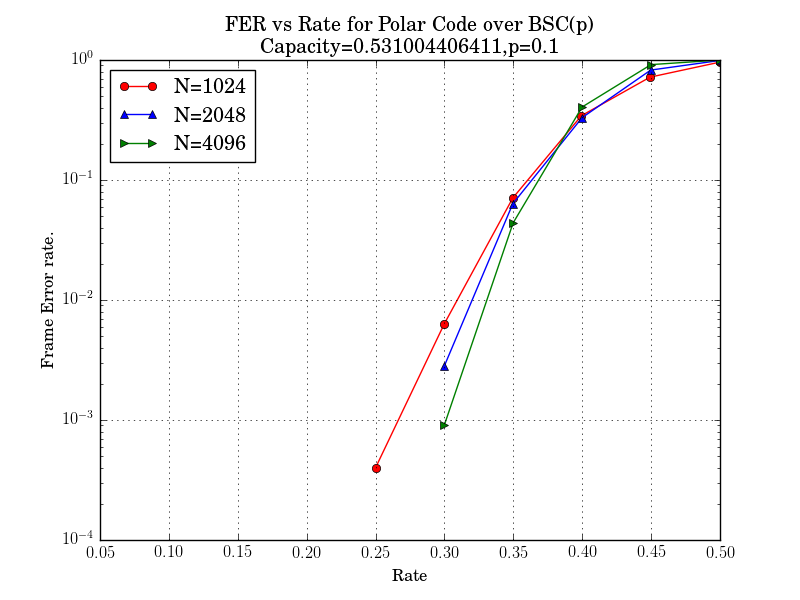
\includegraphics[width=9cm]{./fer.png}
\end{figure}
\hyperback{\hyperlink{polarencodedecode}{\beamerbutton{back}}}
\end{frame}
%---------------------polarsw
\begin{frame}[label = polarswperformance]
\frametitle{Performance of SW compression Polar Codes}
\begin{figure}
\centering
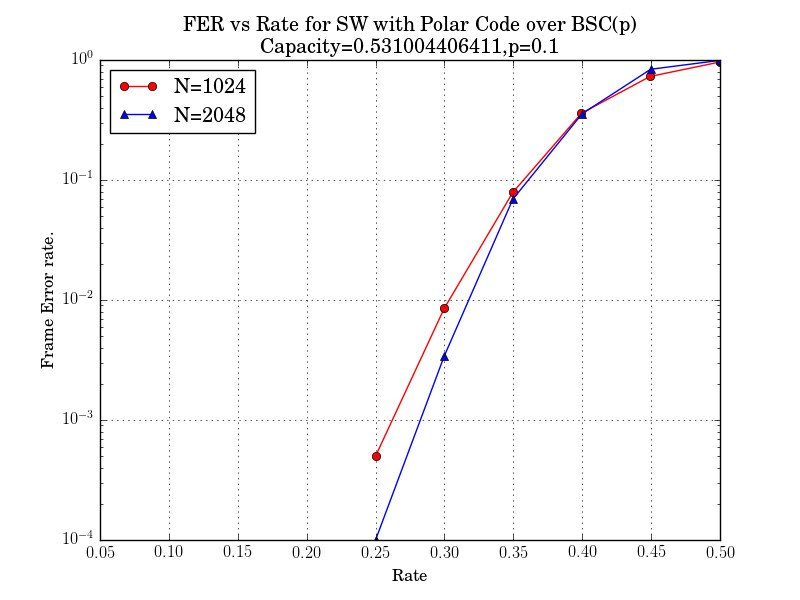
\includegraphics[width=9cm]{./swfer.png}
\end{figure}
\hyperback{\hyperlink{polarslepian}{\beamerbutton{back}}}
\end{frame}
%---------------------selective repetition
\begin{frame}[label = selrep]
\frametitle{Selective Repetition H-ARQ for polar codes}
\begin{columns}
\begin{column}{0.4\textwidth}
\begin{itemize}
\item Initially, an information block of $K$ bits is fed into a polar encoder.
\item The output codeword of $N_0$ bits is punctured into $N_1$
bits and sent over the channel.
\end{itemize}
\end{column}
\begin{column}{0.5\textwidth}
\begin{figure}
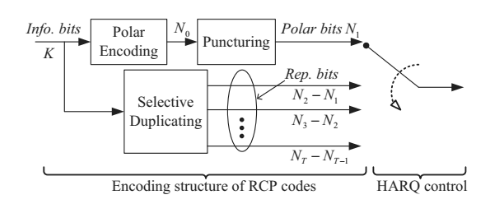
\includegraphics[width=6cm]{./selrepharq.png}
\end{figure}
\end{column}
\end{columns}
\begin{itemize}
\item {Retransmission process}
\begin{itemize}
\item On decoding failure receiver sends a NACK.
\item $N_2-N_1$ of the information bits are retransmitted. 
\item The receiver tries to perform decoding with all the $N_2$ received
bits.
\item This process continues until the transmitter
receives an ACK 
\end{itemize}
\end{itemize}
\vspace{.5cm}
\tiny The retransmitted bits (RV) are chosen one at a time as the most unreliable of the $K$ bits transmitted, reliability is calculated after choosing one bit and the process is iterated. Note, $N_0>...N_3>N_2>N_1$.
\hyperback{\hyperlink{HARQp}{\beamerbutton{back}}}
\end{frame}
%---------------------subset polar
\begin{frame}[label = subpol]
\frametitle{Subset Polar Codes}
\begin{itemize}
\item A Subset Polar Code can be created by greedily puncturing a low-rate mother code without re-optimizing the information bits.
\item The scheme uses equivalent Subset Polar Codes as RV.
\item This has the better performance compared to other HARQ methods.
\end{itemize}
\hyperback{\hyperlink{HARQp}{\beamerbutton{back}}}
\end{frame}
%---------------------RB-HARQ
\begin{frame}[label = rbharq]
\frametitle{Reliability based HARQ}
Reliability based HARQ technique (RBHARQ) , eliminates the use of CRC by approximating bit and word error probability from likelihood ratios (LLR).   The bit error probability for the $k^{th}$ bit can be estimated from LLR ($\tilde{u}_k$) as,
\begin{equation}\label{eq:errorllr}
P_{b,k}=P(\hat{u_k} \neq u_k) = \frac{1}{1+e^{|\tilde{u}_k|}}
\end{equation}
then word error probability becomes, 
\begin{equation}
P_w=1-e^{log\bar{P}_w}
\end{equation}
where, $$log\bar{P}_w=log\prod_{k=1}^K (1- P_{b,k})$$ 
If the word error probability does not meet the requirements the bits with higher bit error probability may be retransmitted. This increases throughput, particularly evident in case of short packet lengths.
\hyperback{\hyperlink{HARQp}{\beamerbutton{back}}}
\end{frame}
%---------------------rcp
\begin{frame}[label = rcp]
\frametitle{Rate Compatible Codes}
\begin{itemize}
\item Given a fixed number of information bits, consider a family of codes $\{C_1,C_2...C_n\}$  with rates $R_1\geq R_2\geq R_3...\geq R_n$, and block lengths $N_1 \leq N_2 \leq ... \leq N_n$.
Then the set is rate compatible if codeword for $C_i$ can be built by removing $N_j-N_i$ bits from codewords of code $C_j$ , $j\geq i$, .
\item Rate Compatible Codes can be constructed by puncturing low rate codes. 
\end{itemize}
\hyperback{\hyperlink{HARQ}{\beamerbutton{back}}}
\end{frame}

%-------------------performance
\begin{frame}[label=pch1]
\frametitle{Performance Evaluation for Inc-Frz/PHY-ED error control coding}
Let $K$ be the number of bit-channels assumed to be good at the first iteration. For simulation, $K$ is varied from $0$ to $K^*$ such that $K^*/N$ is the capacity of the best channel.The scheme uses iterations to communicate these $K$ bits, thus achieving some rate and corresponding frame error rate (FER).
\begin{minipage}[1.1\textheight]{\textwidth}
\begin{columns}
\begin{column}{0.5\textwidth}
\begin{figure}
\centering
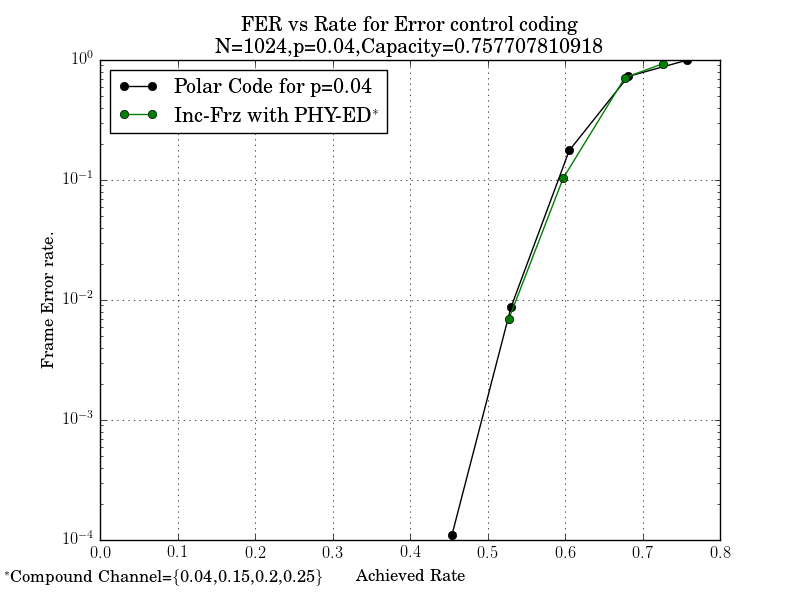
\includegraphics[width=6cm]{./FER_channel0p04.png}
\end{figure}
\end{column}
\begin{column}{0.5\textwidth}
\begin{figure}
\centering
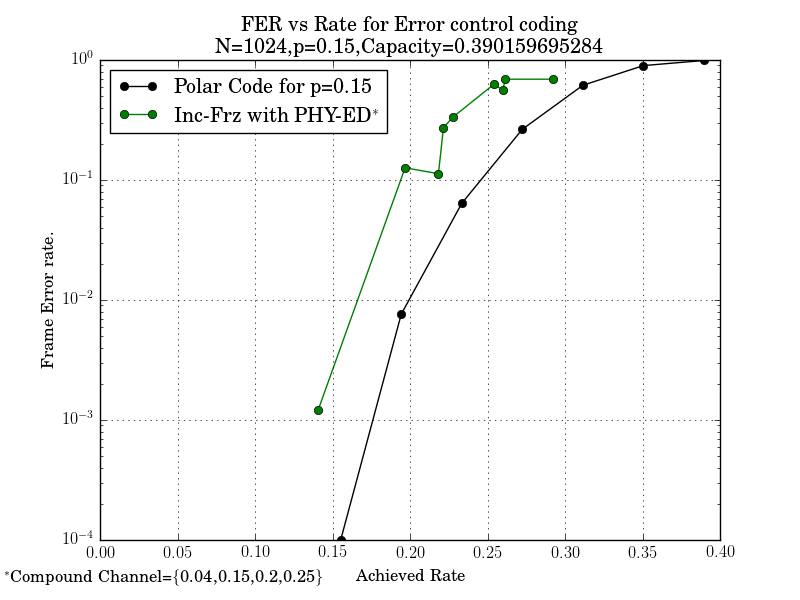
\includegraphics[width=6cm]{./FER_channel0p15.png}
\end{figure}
\end{column}
\end{columns}
\end{minipage}
\hyperback{\hyperlink{psw1}{\beamerbutton{back}}}
\end{frame}

\begin{frame}[label=pch2]
\frametitle{Performance Evaluation for Inc-Frz/PHY-ED error control coding}
\begin{minipage}[1.1\textheight]{\textwidth}
\begin{columns}
\begin{column}{0.5\textwidth}
\begin{figure}
\centering
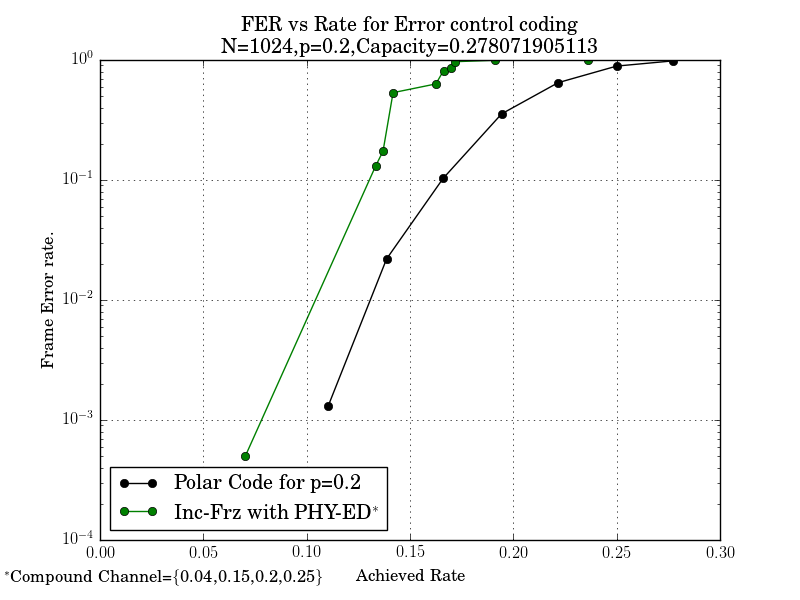
\includegraphics[width=6cm]{./FER_channel0p2.png}
\end{figure}
\end{column}
\begin{column}{0.5\textwidth}
\begin{figure}
\centering
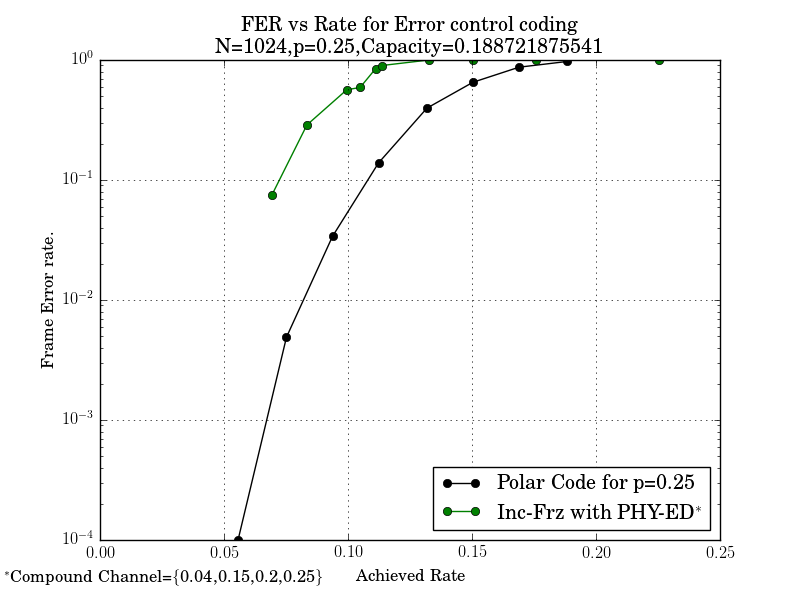
\includegraphics[width=6cm]{./FER_channel0p25.png}
\end{figure}
\end{column}
\end{columns}
\end{minipage}
\hyperback{\hyperlink{psw2}{\beamerbutton{back}}}
\end{frame}

\begin{frame}[label=pch3]
\frametitle{Performance Evaluation for Inc-Frz/PHY-ED error control coding}
\begin{figure}
\centering
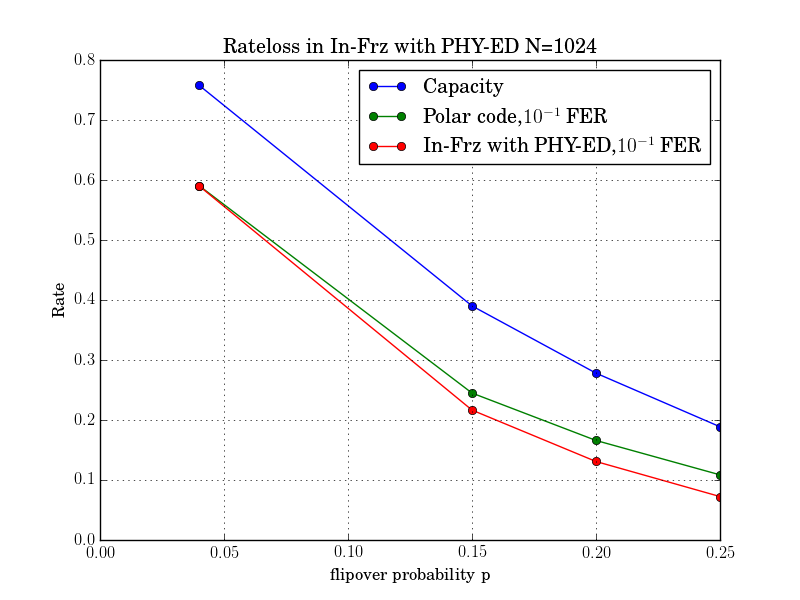
\includegraphics[width=9cm]{./rateloss_channel.png}
\end{figure}
\hyperback{\hyperlink{psw3}{\beamerbutton{back}}}
\end{frame}
%-------------------------------incfrz2
\begin{frame}[label = incfrz2]
\frametitle{Incremental Freezing}
\framesubtitle{continued...}
\begin{itemize}
\item Features
\begin{itemize}
\item By decoding the bits from future transmissions they effectively become frozen.
\item This scheme is capacity achieving in the sense that no rate has been wasted.\footnote{\tiny, Figure illustrates the scheme for a set of channels with rates $\{ R_1=6/8, R_2= R_1/2=3/8,R_3= R_1/3=1/4\}$. After the $3^{rd}$ transmission  $u_2$ to $u_{5}$ have been incrementally frozen. The final rate achieved is, $R^*= \frac{6}{8*3}=\frac{1}{4}=R_3 $}
\item A certain number of channels in this scheme is "\emph{always available}" guaranteeing a certain rate in each transmission. 
\item $n$ iterations of the scheme is almost equivalent in performance to a $R/n$ fixed rate Polar Code.
\end{itemize}
\end{itemize}
\end{frame}

\end{document}